% ============================================================
%  深圳大学实验报告（Python 程序设计 · Project 1）
%  编译方式：XeLaTeX
% ============================================================

\documentclass[a4paper,12pt]{article}

% ----------------------------
% 中文与字体支持
% ----------------------------
\usepackage{fontspec}
\usepackage{xeCJK}
\setCJKmainfont{Noto Serif CJK SC}

% ----------------------------
% 页面设置与常用宏包
% ----------------------------
\usepackage{geometry}
\geometry{left=1in, right=1in, top=1in, bottom=1in}

\usepackage{longtable}
\usepackage{graphicx}
\usepackage{fancyhdr}
\usepackage{tikz}
\usetikzlibrary{calc}
\usepackage{verbatim}
\usepackage{float}
\usepackage{booktabs}
\usepackage{amsmath}

% ============================================================

\begin{document}

% ============================================================
% 封面页
% ============================================================
\begin{titlepage}
    \centering
    \vspace*{2cm}
    \Huge{\textbf{深 \ 圳 \ 大 \ 学 \ 实 \ 验  \ 报 \ 告}}\\[1.5cm]

    {\Large\textbf{课程名称}\quad\underline{\makebox[8cm][c]{Python程序设计}}}\\[0.5cm]
{\Large
\noindent\makebox[3.2cm][l]{\textbf{项目名称}}
\underline{\makebox[8cm][c]{用NumPy复现OpenCLIP图像编码器}}}\\[0.5cm]
{\Large
\noindent\makebox[3.2cm][l]{\textbf{学 \quad \quad 院}}
\underline{\makebox[8cm][c]{人工智能学院}}}\\[0.5cm]
{\Large
\noindent\makebox[3.2cm][l]{\textbf{专 \quad \quad 业}}
\underline{\makebox[8cm][c]{}}}\\[0.5cm]
{\Large
\noindent\makebox[3.2cm][l]{\textbf{指导教师}}
\underline{\makebox[8cm][c]{舒婷}}}\\[0.5cm]
{\Large
\noindent\makebox[3.2cm][l]{\textbf{报 \ 告 \ 人}}
\underline{\makebox[3cm][c]{李振宏}}
\hspace{0.5cm}
\textbf{学号}
\underline{\makebox[3cm][c]{}}}\\[0.5cm]
{\Large
\noindent\makebox[3.2cm][l]{\textbf{实验时间}}
\underline{\makebox[8cm][c]{2026年11月}}}\\[0.5cm]
{\Large
\noindent\makebox[3.2cm][l]{\textbf{提交时间}}
\underline{\makebox[8cm][c]{2026年11月26日}}}\\[1.5cm]

    \vfill
    \Large{\textbf{教务处制}}
\end{titlepage}

\newpage

% ============================================================
% 正文部分
% ============================================================

\section{Objectives}

本次项目的任务是不依赖 PyTorch、OpenCLIP 包和 GPU，只用 NumPy 把 OpenCLIP
ViT-B-32 图像编码器（image tower）的前向计算完整复现出来。模型权重由课程直接提供，
不需要训练，但要求输出与课程给的独立 FP32 参考实现逐阶段数值对齐：
内部 token 序列的容差是 atol=2e-4、rtol=2e-4，最终 512 维输出 token 的容差收紧到
atol=2e-5、rtol=2e-4。

我给自己定的目标比"跑通"多一层：我希望借这个项目把 ViT 的数据流在张量形状层面
真正走一遍。以前读 ViT 论文时，patch embedding、multi-head attention 这些概念
都停留在示意图上；这次必须亲手把 $[B,3,224,224]$ 变到 $[B,49,3072]$ 再变到
$[B,50,768]$，每一个轴是什么含义都得想清楚，否则 reshape 和 transpose 一写就错。
做完之后确实对"多头到底是怎么分的""CLS token 在哪里起作用"有了具体得多的理解。

\section{Overview}

我的实施过程大致分三步：

\begin{enumerate}
    \item[第一步] 先通读附件里的 README、config.json 和 transformer\_steps.py。
    transformer\_steps.py 用三个 token、四个特征的小例子把 Norm、q/k/v、分数、
    系数、残差、MLP 的算术逐步打印出来，我对照幻灯片（46--66 页）把它手推了一遍，
    确认了自己对每一步的理解，尤其是"线性权重按 [out,in] 存储、相乘前要转置"
    这条约定。
    \item[第二步] 按 TODO 的依赖顺序逐个实现：TODO-01（patchify）$\rightarrow$
    TODO-02（split\_heads）$\rightarrow$ TODO-03（注意力）$\rightarrow$
    TODO-04（Transformer block）$\rightarrow$ TODO-05（embed）$\rightarrow$
    TODO-06（输出头）。每填完一组就跑对应的 check.py 阶段，而不是全部写完再测，
    这样一旦出错能立刻定位是哪一步引入的。
    \item[第三步] 八个阶段全部 PASS 之后，用 run.py 对 10 张本地图片批量推理，
    生成 output\_tokens.npz，确认任意输入、任意 batch size 都能正常工作
    （batch 阶段专门检查了乱序和重复图片的一致性）。
\end{enumerate}

模型整体结构如图~\ref{fig:vit-arch} 所示：图像切块线性投影后与 CLS token 拼接、
加上位置编码，经过 12 层 pre-Norm Transformer block，最后取 CLS 位置做 post-Norm、
线性投影到 512 维并归一化。

\begin{figure}[H]
    \centering
    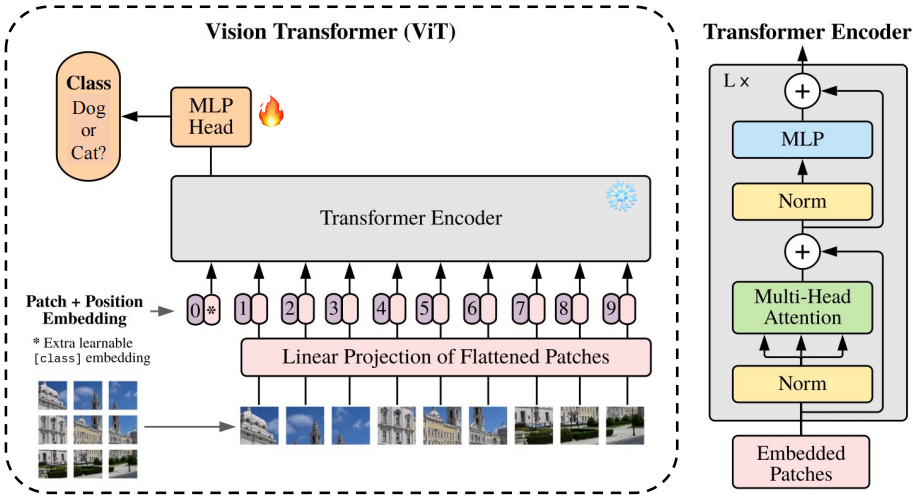
\includegraphics[width=0.92\linewidth]{figs/vit_overview.png}
    \caption{ViT 图像编码器的整体数据流：切块 $\rightarrow$ 线性投影 + CLS + 位置编码
    $\rightarrow$ 12 层 Transformer block $\rightarrow$ 取 CLS 输出投影归一化}
    \label{fig:vit-arch}
\end{figure}

\section{Implementations}

全部改动集中在 image\_encoder.py 一个文件里，下面按模块说关键实现。

\subsection{patchify：从图像到 patch 序列（TODO-01）}

输入是预处理好的 $[B,3,224,224]$。224/32=7，所以每张图有 $7\times7=49$ 个 patch。
我的做法是三步：

\begin{verbatim}
images.reshape(B, 3, 7, 32, 7, 32)      # 拆出网格轴和块内轴
       .transpose(0, 2, 4, 1, 3, 5)     # -> [B, 7, 7, 3, 32, 32]
       .reshape(B, 49, 3072)            # 网格摊平 + C,H,W 摊平
\end{verbatim}

这里最容易犯的错是摊平顺序。patch\_weight 在 \_\_init\_\_ 里已经 reshape 成
$[768, 3072]$，3072 这一个轴的展开顺序是 C,H,W（RGB 三个通道各自 32$\times$32 连续），
所以 transpose 之后轴的排布必须是"网格在前、(C,H,W) 在后"。我一开始写成了
transpose(0, 2, 4, 3, 1, 5)（把 C 放在网格后面、H/W 顺序也乱了），patches 阶段
直接报形状错；后来我换了个办法：先在纸上给六个轴各标一个语义标签，确认 transpose
参数是"新顺序里每个位置取原数组第几个轴"，再落笔，之后就没有再错过。

\subsection{split\_heads 与多头注意力（TODO-02、TODO-03）}

split\_heads 把 $[B,N,768]$ 变成 $[B,12,N,64]$：

\begin{verbatim}
x.reshape(B, N, 12, 64).transpose(0, 2, 1, 3)
\end{verbatim}

课程刻意没有给出多头组织方式的提示，需要自己查资料确定。我查了 PyTorch
MultiheadAttention 的做法并自己验证：特征轴先按 (N, H, head\_dim) 切分、再交换
token 轴和头轴，等价于"第 $i$ 个头拿到特征向量的第 $[64i,\,64i+64)$ 这一段"，
每个头在自己的 64 维子空间里独立做注意力。reshape 必须先于 transpose——如果直接
reshape 成 (B, 12, N, 64)，拿到的就是按 token 顺序切碎的错位数据。

注意力本体（TODO-03）分三小步：

\begin{enumerate}
    \item 分数：$s = qk^{\top}/\sqrt{64}$，其中 $qk^{\top}$ 用
    \verb|q @ k.transpose(0,1,3,2)| 实现，只交换 k 的最后两轴（逐头转置），
    B、H 两个分组轴保持不动；
    \item 系数与加权：softmax 由提供的 attention\_weights 完成，
    \verb|context = coefficients @ v| 得到 $[B,12,N,64]$；
    \item 合并头：transpose 回 $[B,N,12,64]$ 再摊平成 $[B,N,768]$，
    最后做输出投影 \verb|merged @ out_weight.T + out_bias|。
\end{enumerate}

合并这一步和 split\_heads 必须严格互逆：先 transpose 回 (N, H, head\_dim) 再摊平，
摊平顺序才是 (H, head\_dim)，与拆分时的切法一一对应。缩放因子我写成了
\verb|np.float32(np.sqrt(self.head_dim))|：如果直接用 Python float 去除，
NumPy 会把 float32 数组提升成 float64。虽然提升精度后的结果大概率也能过容差，
但我希望整条流水线保持和参考实现一致的 float32 精度，避免引入不必要的系统性偏差。

\subsection{Transformer block 与输出头（TODO-04、TODO-05、TODO-06）}

block 是标准 pre-Norm 结构，两条残差路径：

\begin{verbatim}
residual = x + attention(norm1(x))            # 第一条残差
u = norm2(residual)
mlp = gelu(u @ W1.T + b1) @ W2.T + b2         # [B,N,3072] -> [B,N,768]
return residual + mlp                         # 第二条残差
\end{verbatim}

embed（TODO-05）里 patch 投影没有偏置，直接 \verb|patches @ patch_weight.T|；
CLS 行用 np.tile 复制到 batch 维后放在第 0 行，49 个 patch 行随后，位置编码
$[50,768]$ 对整个序列一次性广播相加。

输出头（TODO-06）对应幻灯片 67--70 页的四步：取第 0 行 CLS（\verb|tokens[:, 0]|，
得到 $[B,768]$）、过 ln\_post、乘 visual.proj（注意这个权重本身就是 [in,out]，
不转置）、最后用提供的 unit\_vector 做单位长度归一化。

\section{Results}

用 \verb|python check.py --stage all| 跑完八个阶段，结果全部 PASS，
各阶段的数值误差记录如下：

\begin{table}[H]
\centering
\caption{各阶段数值校验结果（容差条件：$|actual - ref| \le atol + rtol \cdot |ref|$）}
\begin{tabular}{lcccc}
\toprule
阶段 & 输出形状 & max\_abs & mean\_abs & 容差 (atol) \\
\midrule
assets       & ---            & ---        & ---        & ---   \\
preprocess   & (10,3,224,224) & 0          & 0          & 2e-6  \\
patches      & (2,49,3072)    & 0          & 0          & 2e-4  \\
tokens       & (2,50,768)     & 4.005e-05  & 1.289e-06  & 2e-4  \\
block0       & (2,50,768)     & 7.063e-06  & 3.250e-07  & 2e-4  \\
last\_tokens & (2,50,768)     & 4.768e-05  & 2.696e-06  & 2e-4  \\
output       & (10,512)       & 5.439e-07  & 8.311e-08  & 2e-5  \\
batch        & (3,512)        & 4.619e-07  & 7.632e-08  & 2e-5  \\
\bottomrule
\end{tabular}
\end{table}

几点观察：

\begin{enumerate}
    \item patches 阶段误差为 0，因为切块和投影只涉及数据重排与一次精确的矩阵乘法，
    没有累积误差的来源；preprocess 为 0 则说明它只是逐位复制了预处理结果。
    \item 中间 token（tokens/block0/last\_tokens）误差在 $10^{-5}$ 量级，来自
    12 层 block 中矩阵乘法累加顺序与参考实现（独立 Torch FP32）的细微差异，
    这是浮点非结合性的正常表现，远小于 $2\times10^{-4}$ 的容差。
    \item 最终输出误差反而最小（$10^{-7}$ 量级）：post-Norm 和单位长度归一化把
    向量的整体尺度压掉了，累积的尺度误差被归一化"洗掉"，只剩方向上的微小差异。
    \item batch 阶段复现了乱序加重复图片的组合（顺序 [1,0,1]），第 0 行和第 2 行
    输出一致，说明实现没有混入任何与输入顺序有关的状态。
\end{enumerate}

随后 \verb|python run.py --output output_tokens.npz| 成功保存了
$(10, 512)$ 的输出 token，与输入图片顺序一一对应。

\section{Discussion}

\subsection{修复过的一个 bug}

填 TODO-03 的时候我出过一个比较典型的错误：当时把 scores 的计算直接插在了
TODO-03a 的注释位置，但那段代码引用的 q、k 是在注释上方几行才定义的——我整理
代码时把 qkv 计算挪到了 scores 后面，运行直接 NameError。排查时我以为是自己
split\_heads 写错了，对着 transpose 参数检查了半天，最后才发现只是语句顺序问题。
这事的教训是：往带 TODO 的骨架里插代码时，要先看清"Given"注释和变量的依赖关系，
不要只看 TODO 标记的位置。之后我养成了习惯，每填完一个 TODO 先跑最小阶段的校验
（check.py 的分阶段设计确实帮了大忙），错误永远不会离引入它的地方太远。

\subsection{一次形状变化的理解：split\_heads}

我认为整个项目里最值得讲清楚的形状变化是 split\_heads。
$[B,N,768]$ 到 $[B,12,N,64]$ 的变换分两步，两步的顺序不能换：
reshape(B, N, 12, 64) 把特征轴切成 12 段，这一步在内存里不搬数据，只是换个视角；
transpose(0, 2, 1, 3) 才真正交换 token 轴和头轴，让每个头可以独立地对自己那片
$[N,64]$ 的 q/k/v 做矩阵乘。反过来的合并（merge heads）必须完全对称：
先 transpose 回 $[B,N,12,64]$ 再 reshape 成 $[B,N,768]$。我曾经想当然地直接从
$[B,12,N,64]$ reshape 成 $[B,N,768]$，那样等于把 12 个头的输出按错误的交错顺序
缝回去——虽然形状恰好对，数值完全是错的。check.py 用真实权重一测就暴露了，
这也让我体会到"形状对不等于实现对"。

\subsection{性能观察与改进想法}

课程提供的 GELU 为了保证逐位精确，用 Python for 循环逐元素调用 math.erf。
我算了一下开销：MLP 中间层是 $[B,50,3072]$，B=10 时单层约 1536 万个元素，
12 层合计约 1.8 亿次 erf 调用，跑一次 output 校验要等好几分钟。这是本次实验
最明显的性能瓶颈。如果想提速，可以把循环换成 scipy.special.erf 的向量化调用
（同一数学定义，误差在 $10^{-7}$ 量级，先在 block0 阶段对齐验证后再全局替换），
预计能快两个数量级；不过考虑到课程要求与参考实现严格对齐，我最终保留了原始实现，
只在报告里记录这个权衡。

其他可以改进的点：一是注意力部分可以用 np.einsum 写得更紧凑，
\verb|einsum('bhqd,bhkd->bhqk', q, k)| 的语义比 transpose(0,1,3,2) 更直白；
二是 patch 投影等价于一个 stride=32 的卷积，权重 reshape(768,3072) 的做法
提示了 conv1.weight 原始布局是 $[768,3,32,32]$，理解这一点对复用进期末项目
的文本塔有帮助；三是目前每个 block 每次前向都重复做 \verb|weight.T|，
如果要反复推理可以把转置缓存到 \_\_init\_\_ 里，代价是内存翻倍，这里按课程
"参数保持不动"的约定没有做。

\subsection{环境问题记录}

实验中还遇到一个和模型无关但耗时不少的问题：我机器上有多个 Python
（3.11/3.13/3.14），其中默认的 3.11 是非标准安装，site-packages 没有出现在
sys.path 里，pip 装好的 numpy 在脚本模式下导入失败。排查了 sys.path 和
py launcher 注册表之后，我临时用 PYTHONPATH 指向 site-packages 解决。
这个问题让我意识到 Python 环境混乱是"跑别人的项目"最常见的隐性成本，
以后遇到 ImportError 应该先打 \verb|sys.executable| 和 \verb|sys.path|，
而不是急着重装依赖。

\subsection{协助说明}

TODO 部分的实现、调试和本报告由本人完成。过程中借助 AI 助手做了两件事：
一是排查上述 Windows 多解释器的模块导入问题，二是在我拿不准 transpose 轴序时
帮我核对 NumPy 文档里 transpose 参数的语义（"新顺序下各轴来自原数组的第几个轴"）。
split\_heads 的多头组织方式我先自行查了 PyTorch MultiheadAttention 的文档和
社区讨论，再用小数组手工验证后才写入代码。代码中所有关键步骤都附有我自己的
中文注释，便于面试时逐行解释。

\newpage

% ============================================================
% 批阅与成绩评定页
% ============================================================

\begin{tikzpicture}[remember picture, overlay]
  \draw[thick]
    ($(current page.north west)+(2cm,-3cm)$)
    rectangle
    ($(current page.south east)+(-2cm,3.5cm)$);
\end{tikzpicture}

\vspace{1cm}

\noindent \textbf{指导教师批阅意见：}
\vspace{6cm}
\hfill

\vspace{1cm}

\noindent \textbf{成绩评定：}
\vspace{2cm}
\hfill

\vspace{1cm}

\noindent
\hfill
\textbf{指导教师签字：}\quad\quad\quad\quad\quad\\[0.5cm]

\hfill
\textbf{年}\quad\quad
\textbf{月}\quad\quad
\textbf{日}\quad

\vspace{1cm}

\noindent \textbf{备注：}

\begin{tikzpicture}[remember picture, overlay]
  \node[
    anchor=north west,
    inner sep=0pt,
    text width=\dimexpr\paperwidth-4cm\relax
  ] at ($(current page.south west)+(2cm,3.1cm)$) {
    \begin{minipage}{\dimexpr\paperwidth-4cm\relax}
      \small
      \noindent
      \textbf{注：}\;1、报告内的项目或内容设置，可根据实际情况加以调整和补充。\\[0.2cm]
      \phantom{\textbf{注：}\;}2、教师批改学生实验报告时间应在学生提交实验报告时间后 10 日内。
    \end{minipage}
  };
\end{tikzpicture}

\end{document}
